\documentclass[sigchi]{acmart}
\usepackage{algorithm}
\usepackage[noend]{algpseudocode}

\AtBeginDocument{%
  \providecommand\BibTeX{{%
    \normalfont B\kern-0.5em{\scshape i\kern-0.25em b}\kern-0.8em\TeX}}}

\settopmatter{printacmref=false, printccs=false, printfolios =false}
\setcopyright{none} 
\renewcommand\footnotetextcopyrightpermission[1]{}

\acmConference[SDCC Project A.A. 2018-2019]{ }{September 18, 2019}{ }

\begin{document}

\title{Byzantine Fault-Tolerant and Locality-Aware Scheduling MapReduce}

\author{Andrea Graziani}
\email{andrea.graziani93@outlook.it}
\affiliation{%
  \institution{Università Degli Studi di Roma Tor Vergata}
  \city{Rome}
  \state{Italy}
}

\renewcommand{\shortauthors}{Andrea Graziani (0273395)}





\begin{abstract}
\textit{MapReduce} is a programming paradigm developed by Google that enables massive scalability across hundreds or thousands of servers allowing to process very large data-set \cite{IBMWhatIsMapReduce}.

Both academic literature and daily experience shows that \textit{arbitrary faults} frequently occur corrupting our results \cite{BFLMapReduce}. Moreover, ignore \textit{data-set locality} can lead to performance degradation and a pointless bigger network traffic \cite{LARTS}.

In this paper we present a MapReduce runtime system as a solution to these problems. Although job's execution using our system requires more resources respect to other implementations due to process replications, we believe that this cost is acceptable for critical applications that require an higher level of fault tolerance.
\end{abstract}

\keywords{MapReduce, Arbitrary Fault Tolerance, Locality Awareness, Speculative Execution, Leader Election Algorithm, Deferred Execution}
\maketitle

\section{Introduction}

Various data-intensive tasks, like seismic simulation, natural language processing, machine learning, astronomical data parsing, web data mining and many others, require a processing power that exceeds the capabilities of individual computers imposing the use of a \textit{distributed computing} \cite{LARTS}.

Nowadays many famous distributed applications use MapReduce framework as solution for processing large data sets in a distributed environment. In order to properly provide services to an increasing number of users worldwide, is necessary to connect together thousands of computers and hundreds of other devices like network switches, routers and power units, moving consequently an huge amount of data between computers. 

However, as many studies confirm, \textit{hardware component failures are frequent} and they will probably happen more often in the future due to increasing number of computers connected to internet \citep{BFLMapReduce}. Is been documented that in the first year of a cluster at Google there were 1000 individual machine failures and thousands of hard drive failures \cite{PetaScaleFailure}. A recent study of DRAM errors in a large number of servers in Google data-centres for 2.5 years concluded that these errors are more prevalent than previously believed, with more than 8\% DIMM affected by errors yearly, even if protected by error correcting codes (ECC) \cite{DRAMError}. A Microsoft study of 1 million consumer PCs shown that CPU and core chipset faults are also frequent \cite{MicrosoftStudyFailure}. Moreover moving large amount of data repeatedly among distant nodes is becoming the bottleneck owing to an increased network traffic, causing significant performance degradation.

For these reasons, to construct a distributed system capable to provide its services even in the presence of failures, mitigating network traffic and delay, is become a critical aspect of software engineering.

In these paper we will describe an \textit{Arbitrary Fault-Tolerant Locality-Aware} (AFT-LA) MapReduce system capable to resolve all issues described above. 

\begin{table*}
  \caption{Libraries used in our implementation}
  \label{tab:libraries}
  \begin{tabular}{l|l|l}
    \toprule
    Name & Description & Link \\
    \midrule
    \texttt{go-zookeeper/go} & Native Go Zookeeper Client Library & \url{https://github.com/samuel/go-zookeeper} \\
    \texttt{logrus} & A structured logger for Go & \url{https://github.com/Sirupsen/logrus} \\
    \texttt{aws-sdk-go} & AWS SDK for the Go programming language. & \url{https://github.com/aws/aws-sdk-go} \\
    \bottomrule
  \end{tabular}
\end{table*}

\section{Assumptions and remark}

In order to properly describe how our system can achieve a certain level of arbitrary fault tolerance without unduly compromising performance, let's start making some very important assumptions and observations.

We have designed our cloud application as a \textit{set of processes}, every of which have to both run on \textit{different} servers and have got a certain replication degree in order to achieve a certain level of arbitrary fault tolerance, therefore we have deploy our processes in several Amazon EC2 instances hosted in a same region (\texttt{us-east-1})\footnote{Note that, due to Account AWS Educate Starter limitations, we couldn't run Amazon EC2 instances on other regions.}.

In order to enable communication with the Internet and therefore allow a local computer to connect to our system, we have adopt AWS Elastic IP\footnote{\url{https://docs.aws.amazon.com/en_us/AWSEC2/latest/UserGuide/elastic-ip-addresses-eip.html}} which able us to associate to some of our EC2 instance to a public static IPv4 addresses\footnote{Public IPv4 addresses associated to any EC2 instances by default change after every start. Therefore, if an Amazon EC2 crashed and have to be restarted, client wouldn't able to connect to it due to address change.}.

Observe that processes are not all the same but several kind of these exist, with its own features and aims: although we will describe them in detail in following section, just note that we distinguish three process type: \textit{Client Process}, \textit{Primary Process} (PP) and \textit{Worker Process} (WP); 

Note that our MapReduce system is been implemented to execute word-count job only. We have built our system from scratch using Go programming language\footnote{\url{https://golang.org}} using some external libraries, which are all reported in table \ref{tab:libraries}. 

We assume that our system runs \textit{asynchronously}, that is no assumptions about process execution speeds or message delivery times are made; therefore we can normally use a time-out to state that a process has crashed although, occasionally, such conclusion is false \cite{SDCC}.

All processes are connected by \textit{reliable channels}, that is no messages are lost, duplicated or corrupted. In our prototype that feature is guaranteed  by the use of Go implementation of RPC\footnote{\url{https://golang.org/pkg/net/rpc/}} (\textit{Remote Procedure Call}) which is based on TCP connections. Mostly all RPC calls, except those made by the client process, are asynchronous\footnote{Although Go's \texttt{rpc} package provides its own support for RPC asynchronous calls, we have  preferred to adopt an equivalent approach based on properly used goroutine and channels.}.

Clients are \textit{always correct}, because if they are not there is no point in worrying about the correctness of our system's output. We assume the existence of an hash function that is \textit{collisions-resistant}, for which it is infeasible to find two inputs that produce the same output.

Finally, we remember that our prototype's source code is fully available on GitHub\footnote{\url{https://github.com/AndreaG93/SDCC-Project}}, famous web-based hosting service for version control using \texttt{git}; we remind that \LaTeX\ source code of this paper is available too\footnote{See \url{https://github.com/AndreaG93/SDCC-Project-Report}}. In this paper, we take for granted reader's knowledge of the MapReduce framework and part of Hadoop framework.

\section{System's model}

Let's start now the analysis of all processes of our system.

\begin{figure}[h]
  \centering
  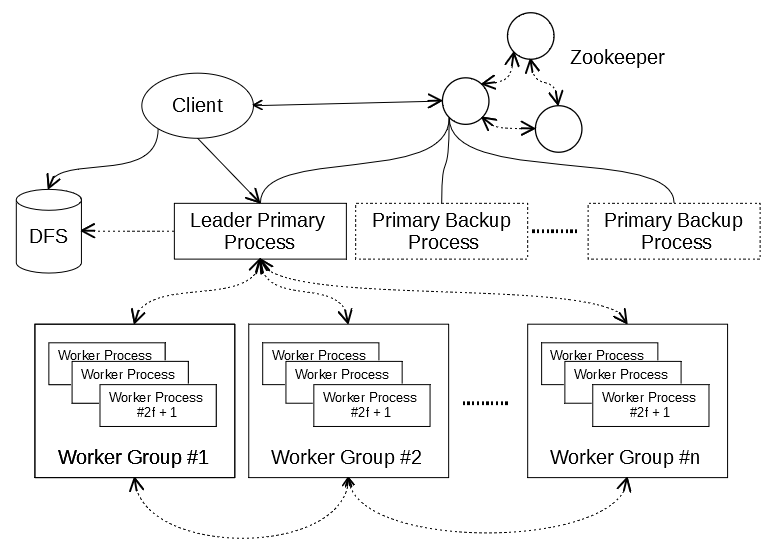
\includegraphics[width=\linewidth]{Architecture.png}
  \caption{System Architecture}
  \label{fig:model}
\end{figure}

\subsection{Client Process}

This process, which, as said previously, is assumed always correct, is the place where (word-count) jobs are submitted to our system. 

It can interact with system's key-value storage service (i.e. DFS or an equivalently cloud key-value storage service) for job's input uploading and job's output downloading. To perform data transmissions, client processes use HTTP-based RESTful APIs, according to which both an URL and standard HTTP methods (\texttt{GET} and \texttt{PUT}) only are required.

Is very important to specify that, in our system, URLs are provided by a PP for security and compatibility reasons with some cloud storage services. In fact, unlike Hadoop, which use HDFS (\textit{Hadoop Distributed File System}) to store input and output data, our prototype adopts Amazon S3 for data storage purposes. According to Amazon S3 implementation, since all objects and directories (\textit{buckets}) are by default private, clients cannot upload or download data without AWS security credentials or permissions.

Therefore, rather than distribute AWS security credentials which can imply huge security risks, we have adopt a design according to which client processes have to request special URLs to PP to accomplish their data transmissions; these kind of URLs are called \textit{pre-signed URLs}. According to Amazon AWS documentation, anyone who receives a valid pre-signed URL can upload (or download) an object from Amazon S3. However only someone that has a valid security credentials can create a pre-signed URL; this is the reason according to which PP, that has AWS security credentials to interact with Amazon S3\footnote{We remember that to give all privileges required for pre-signed URL creation to the EC2 instances where PP is running, we have to properly set all necessary IAM Roles thought "\textit{AWS Identity and Access Management service}" (IAM)}, has to generate and distribute them to clients.

Observe that client processes are unaware of PP network location, that is they doesn't know its internet address (which can change during system activities due to either a crash or connectivity lost because to Amazon EC2 policies). To be more precise any system's process know network location of the others although an Apache Zookeeper\textsuperscript{TM}\ cluster location, which we have adopt for membership managing and coordination purposes, must be known by everyone. According to our design, is possible to know network location of a specified process querying Zookeeper cluster, therefore clients are able to know where PP is and then it can both require pre-signed URL and submit jobs.

\subsection{Primary Process}

Most of the activities carried out by a Primary Process are very similar to those performed by \textit{JobTracker} process used in Apache Hadoop framework. These activities including \textit{Map-Task} or \textit{Reduce-Task} scheduling, pre-signed URLs generation, managing of worker nodes replies, clients request managing and so on.

However unlike Apache Hadoop framework, according to which \textit{JobTracker} process is assumed always correct, we have design our system believing that the host where PP is running may fail, for example by crashing or by losing network connectivity; in other words, as known in academic literature, PP represents for us a \textit{single point of failure}. Therefore, to ensure an high system availability, inspired by Apache Mesos\textsuperscript{TM}\ architecture\footnote{See \url{http://mesos.apache.org/documentation/latest/architecture/}}, we have adopt a design according to which multiple PP backup copies exist and they run on \textit{different machines} (in our prototype, on different EC2 instances); using a leader election algorithm, is possible to elect one of these copies as leader, becoming the \textit{Leader Primary Process} (LPP), while all the others remain on stand-by. Using this approach, is possible to manage a PP crash failure: when current LPP fails, a backup copy is promoted to become the new leader. 

Is very important to specify that LPP status is stored in memory, therefore they are permanently lost after a crash; this design makes our system easier to implement and helps to reducing overhead due to the disk I/O activities. However recover lost in-memory leader state after a failure is required in order to satisfy clients requests. 

Therefore we have adopt a design according to which LPP save its state regularly. Since LPP state consists on a very small amount of data, we have design LPP to store its state into Apache Zookeeper cluster upon the occurrence of certain events. When a LPP crash failure occurs, the new leader can easily retrieves last saved state from  ZooKeeper cluster. Note that Apache Zookeeper's processes is been replicated too in order to tolerate a certain number of faults upon Zookeeper cluster.

Another difference Hadoop \textit{JobTracker} process regards task scheduling approach. In our design LPP schedules tasks to WP using a \textit{push-based} approach, contrariwise Hadoop JobTracker schedules task using a \textit{pull-based} approach where WP ask for tasks\cite{LARTS}.

\subsection{Worker Process and Groups}

To achieve fault tolerance we have adopt a design according to which each task is executed more than once by different processes running on different host. To do this, as you can see from figure \ref{fig:model}, we have adopt a design according to which all worker processes are organized in several groups which we have used to mask one or more faulty processes: these groups are called \textit{Worker Processes Group} (WPG). To be more precise, an WPG is a set of identical WP, each of which execute \textit{the same commands using the same input data in the same order}; therefore we expected that all WPs belonging to a same group would produce the same output when no arbitrary fault occurs. 

According to our system's design, any word-count job is made up of two main phases: \textit{Map-Phase} and \textit{Reduce-Phase}. To fully complete the Map-Phase of a job is necessary to successfully perform a certain number of special tasks called \textit{Arbitrary Fault-Tolerant Map-Tasks} (\textit{AFT-Map Tasks}): a AFT-Map represents a fault tolerant version of classical map task, in fact it simply consist on a replicated map task among a certain number of WP. To be more precise, our system is been design so that each WPG performs its own AFT-Map Task independently: to do that, each WPs, belonging to a given WPG, will perform the same map task in order to mask faulty processes. Clearly all this is also valid for Reduce-Phase.

Suppose now to want tolerate at most $f$ arbitrary failures. To achieve that level of fault-tolerance is clearly necessary that any AFT-Map Task or AFT-Reduce Task assigned to each WPG are able to tolerate at most $f$ arbitrary failures. At this point we can apply, for instance, \textit{byzantine agreement} among all processes of a given WPG, but we believe that solution is too expensive because it requires, as properly explain in literature\citep{SDCC}, $3f + 1$ replicas.

Therefore we have adopt a protocol based on \textit{majority voting} inspired to quorum-based protocols applied in replicated-write systems. As explained in literature\citep{SDCC}, in this kind of systems, if processes exhibit arbitrary failures, continuing to run when faulty and sending out erroneous or random replies, a minimum of $2f+1$ processes are needed to achieve $f$-fault tolerance. In the worst case, the $f$ failing processes could accidentally generate the same reply. However, the remaining $f+1$ will also produce the same answer, so the LPP just believes the majority.

Formally, let $i = 1,2,3...n$, where $n \in \mathbb{Z}_+$. LPP splits the input text file $S$ in $n$ parts $\lbrace s_1, s_2, ... s_n \rbrace$ called \textit{splits}; each split $s_i$ is associated to an AFT-Map Task $m_i \in \lbrace m_1, m_2, ... m_n \rbrace$. Each AFT-Map Task $m_i$ is assigned to WPG $g_i \in \lbrace g_1, g_2, ... g_n \rbrace$. Then $2f+1$ different WPs belonging to WPG $g_i$ perform the same map task replica. LPP, checking received outputs from each WP of each group, picks the most voted results which is expected correct if no more than $f$ arbitrary faults occur. Obviously Reduce-Phase is performed in similar ways.

Clearly, this design require more resources respect to classic MapReduce scheme: to tolerate at most $f$ arbitrary failures, each WPG have to contains at least $2f+1$ different WPs, therefore a total of $n(2f+1)$ different WPs are required (to which is also added a certain number of PPs run on different machine).

Although its very high costs, this design is scalable in several ways: if the number of users or data input size grows, it should be possible to extend the system, at reasonable cost, adding more WPGs. If we want an higher level of arbitrary fault-tolerance, we should add more WP to each WPG (increasing the number of PP backups too).

\section{System features}

At this point high costs of this solution should be clear to reader because everything is replicated $2f + 1$ times as map/reduce task, data transmissions and so on. Can we have a good level of fault tolerance without worsening performance? How can we do AFT-Map Task and AFT-Reduce Task efficiently? 

In this section we will explain a set of solutions and techniques which we have adopt in our system to reduce costs and do things efficiently:

\subsection{Digest outputs} As explained above, in order to consider any AFT-Map Task/AFT-Reduce Task correct, tolerating at most $f$ faulty processes, $f + 1$ matching outputs, coming from at least $2f + 1$ WPs belonging to a given WPG to which we have assign the aforementioned task, have to be received. 

Since outputs computed by WPs can be very large, we have adopted an approach according to which, instead of to compare raw data, LPP fetches and compares \textit{digests} that is fixed size strings obtained from WPs outputs using an hash function. The main advantage of this technique is that digest size are many times smaller than task's data output, allowing us to validate task's output reducing network traffic among servers.

\subsection{Locality-And-State-Aware Deferred Execution} 

Waiting for $2f + 1$ matching replies during any AFT Map-Task/AFT-Reduce Task can be a waste of time especially when no faults occur or we have already received a sufficient number of reply to establish the output's correctness; in other words, we believe that there is no point in always executing $2f + 1$ replicas for a given AFT-Map Task/AFT-Reduce Task.

Therefore, to minimize both the number of replicas executed and the overhead due to network traffic, we have adopted a mechanism that we have called \textit{Locality-Aware Deferred Execution}. 

According to that solution, during a AFT Map-Task/AFT-Reduce Task execution, only $f + 1$ replicas are started checking if they all return the same result. If a time-out elapses or some return results do not match, more replicas (up to $f$) are started, until we obtain $f + 1$ matching replies. When faults are unlikely, this approach, which we believe to be energy-saver\footnote{Assuming that idle WPs consume less energy respect to non-idle WPs, minimize the number of Map-Task executed involves minimize the amount of electricity used.}, is capable to minimize the number of WPs involved into computations respect to basic scheme, improving overall system performance.

Moreover, this mechanism can reduce overall system response time because it is designed to minimize data transfer time too because our scheduler gives priority to \textit{nearest} WPs. When an AFT-Map Task/AFT-Reduce Task starts $f + 1$ replica on WPs, the latter are not chosen at random but according to their network location; in fact, the tasks are scheduled firstly to the $f + 1$ nearest nodes. Only when we can't get $f + 1$ matching replies, the most distant nodes are used. The most difficult problem consists into determine WP's network location considering the variation of network traffic. In literature, many network proximity evaluation's methods exist which can be static (i.e. hop number) or dynamic (round-trip time evaluation, HTTP request emulation, etc.); in our prototype, we have adopt a very simple network proximity evaluation's method based on \texttt{ping} which able us to evaluate round-trip time among system's nodes. 

We have designed our task scheduler to be also \textit{state-aware} since priority is given to those WPs whit minimum CPU utilization which we compute using \texttt{mpstat} tool. WP's state is acquired indirectly by LPP through their replies.

\subsection{Speculative Execution}

Although the advantages of the deferred execution mechanism describes above, we believe that waiting for $f + 1$ matching digest for all AFT Map-Tasks before starting the Reduce-Phase can worsen the time for the job completion, especially when WPs arbitrary failures are uncommon. Remember that, assuming that we have $n$ WPGs, since we need at least $f + 1$ matching reply from each WPG, we have to wait for at least $n(f + 1)$ replies; all Map-Phase may require long time due, for instance, to network traffic or big  data-set.

A way to increase system's performance reducing its response time is the following: when all $n$ scheduled AFT Map-Tasks have received the \textit{first} replica's result, LPP starts Reduce-Phase immediately without waiting for each AFT Map-Tasks receive exactly $f + 1$ matching results; in other words, Reduce-Phase starts after one replica of all AFT Map-Tasks finish. Essentially, our system make a bet according to which arbitrary faults are highly unlikely therefore first Map-Task replies are considered as correct. This mechanism is known in literature called \textit{Speculative Execution}, an optimization technique applied frequently in computer technology.

Obviously validate the correctness of first Map-Task replies is critical otherwise job's output can be incorrect. To do that, all scheduled AFT Map-Tasks keep on waiting their $f + 1$ matching replies even when Reduce-Phase is started. When Map-Phase is fully finish, if is detected that the input used in the Reduce-Phase was not correct, Reduce-Phase will be restarted with the correct input, otherwise we can finish our job in much less time.

Then, when there are no fault or they are unlikely, this design is capable to reduce considerably system's response time. 

\subsection{Data-Locality-Aware Reduce Scheduling and Shuffle}

So far we have not yet mentioned the shuffle task according to which WP redistribute data (produced by the map function), such that all data belonging to one key is located on the same WP's node. Unlike Hadoop implementation, shuffle task is difficult and expensive due to process replication and to optimization technique described so far. Clearly, due to process replication, data transfers among servers are replicated too, generating an huge amount of network traffic. Evidently, when large data set are involved, move data repeatedly among server became a bottleneck. 

Therefore we have adopted a design aware of data locations capable to reduce the overall amount of transferred data: this approach is called \textit{Data-Locality-Aware Reduce Scheduling}. That solution is based on a basic principles which states that "\textit{moving computation towards data is cheaper than moving data towards computation}"; in other words  "\textit{moving computation towards data is cheaper than moving data towards computation}".

Using the same Hadoop terminology, map task output, produces by every WPs, are called \textit{partition} and, contrary to splits, they are of variable sizes: so why not just shuffle smaller partitions instead big one? Then, why not schedule a AFT-Reduce Task to the WPG which nodes has bigger partition? In this way we can avoid transferring huge amount of data increasing overall system performances.

To explain how our scheduler works, let's illustrate an example: assume for simplicity to have only two WPGs $\lbrace g_1, g_2 \rbrace$. Let $P_{i:g_i}$ the partition owned by WPG $g_i$ which contains all key-value pairs which must be submitted to reduce task $R_i$. Suppose that $P_{1:g_1}$, $P_{2:g_1}$, $P_{1:g_2}$ and $P_{2:g_2}$ have a size of 300 MB, 150 MB, 150 MB and 300 MB respectively. In this context LPP schedules $R_1$ to $g_1$ and $R_2$ to $g_2$ because in this way is able to reduce transferred data among WPGs by 50\%. In other words, LPP is design to schedule AFT-Reduce Tasks reducing overall amount of shuffled data.

\subsection{Crash failure detection} To guarantee the correct functioning of the system, is critical to be able to detect WP and PP crash failure. To resolve this problem we have exploited some features of Apache Zookeeper. 

As known, Apache ZooKeeper has the notion of \textit{ephemeral nodes}, special znodes which exists as long as the \textit{session} that created the znode is active. When session expiration occurs, Zookeeper cluster will delete all ephemeral nodes owned by that session and immediately notify all connected clients of the change.

When any client establishes a session with a Zookeeper cluster, a time-out value is used by the cluster to determine when the client's session expires. Expirations usually happens when the cluster does not hear from the client within the specified session time-out period (i.e. no heartbeat).

Therefore using that feature, we adopted a very simple design according to which any process must to "sign up" creating his own ephemeral node in Zookeeper Cluster in known paths (note that znode paths of PPs and WPs are different in order to not interfere with leader election of PPs). 

It will be the responsibility of LPP to watch for WP's ephemeral node deletions; this approach makes WP status checking very simple. System coordination and membership is facilitated too, since any ephemeral node is used to store information about process that created (ID, Group ID etc.).


\subsection{Primary process leader election algorithm}

\begin{algorithm}
\caption{}\label{alg:leaderElection}
\begin{enumerate}

\item Let \texttt{ROOT} be a valid znode path. Any PP, which wants to become leader, creates a new znode $Z$ with path \texttt{ROOT/$x$}, where $x$ is a number. Using both \texttt{SEQUENCE} and \texttt{EPHEMERAL} flags, $x$ will be the sequence number greater than any one previously used.

\item Let $C$ be the children of \texttt{ROOT}. 

\item If $Z$ is the smallest node in $C$, that is $x$ is the smallest sequence number used so far, then the PP that created $Z$ will become leader.

\begin{enumerate}

\item Otherwise watch for changes on znode \texttt{ROOT/$j$} in C, where $j$ is the largest sequence number such that $j$ < $x$.

\item Upon receiving a notification of znode deletion, go to step number 2. 

\end{enumerate}
\end{enumerate}
\end{algorithm}

Let's now describe in details how we have resolved leader election problem of a PP using Apache Zookeeper.

Suppose that \texttt{ROOT} is a valid path of an existing znode. To apply as possible leader, any PP creates a znode child into \texttt{ROOT} using \texttt{SEQUENCE} and \texttt{EPHEMERAL} flags. When \texttt{SEQUENCE} is used, ZooKeeper cluster automatically appends a sequence number to the new znode that is greater than any one previously appended to a child of \texttt{ROOT}. The PP, which created the znode with the smallest appended sequence number, become leader.

Obliviously is important to watch for failures of the leader in a such way that a new PP arises as the new leader when leader fails. Note that, since we have used \texttt{EPHEMERAL} flag during znode creation, when leader fails the smallest znode will be deleted by Zookeeper cluster. if we make sure that all PPs watch for the next znode down on the sequence of znodes, if a PP receives a notification that the znode it is watching is gone, then it becomes the new leader since there is no smaller znode. 

A complete description of leader election algorithm is shown in Algorithm \ref{alg:leaderElection} while our implementation is in \texttt{SDCC-Project/aftmapreduce/cloud/zookeeper}

\section{The algorithm}

In this section we will provide a detailed description of our MapReduce algorithm used to fully accomplish any client's word-count request. Our algorithm is made up of five phases every of which have to be successfully completed in order to complete a request.

\subsection{Data upload phase}

The first phase of our algorithm expects that client would upload their test input file into a DFS (\textit{Distributed File System)} or, equivalently, into an external storage service.



\subsection{Acceptance phase}

After data upload, client sends a word-count request to current LPP. 

When that request is been received, LPP, after to have written into Zookeeper cluster all necessary information  in order restore its state after a crash failure (request's status information, text input data digest etc.),  notifies client that his request is been accepted by system, starting Map phase.

When LPP response is been received, client starts to wait for a new notification by Zookeeper cluster (watching a specified znode) which will signalize computation completion.

If any error occurs during this phase, client have to re-forward its request to LPP until it will receive acceptance confirmation. 

Note that our system is able to manage duplicated requests because we have adopted a \textit{most-once semantics}; in fact, LPP is able to recognize duplicates re-forwarding its reply to client while client, if it detects that LPP is been crashed, forwards a query to Zookeeper cluster in order to know who is the new LPP.

\subsection{Map phase}

LPP splits received text into $n$ splits where $n$ is the number of WPGs currently available in the cluster (this number is checked at runtime). Then LPP starts \textit{Map Phase} during which $n$ \textit{Arbitrary-Fault-Tolerant Map Tasks} (AFT-MTs) are initialized and assigned to every WPGs (note that each WPG manages a different AFT-MT). 

To make this phase fault tolerant, each AFT-MT is replicated using the WPs available into a WPG specified by LPP. As explain in previous sections deferred execution and digest outputs are used. Our prototype is designed to check at runtime the number of currently available WPs into a WPG calculating automatically fault tolerance level (for example if there are three WP currently on-line of a specified group, the system behaves properly in order to tolerate one arbitrary failure).

When all AFT-MTs finish successfully, LPP perform a checkpoint storing into Zookeeper cluster a set of meta-data used to restore LPP status in case of crash (these data include digest outputs from WPGs and some information about computed data outputs owned by WPGs). 

In case of LPP crash (note that also an high amount of arbitrary fails of WPs determines a LPP crash), after using our leader election algorithm, a PP backup copy becomes leader. Then the new leader recovers previous leader's status from last checkpoint querying Zookeeper cluster. All pending requests are restarted according to last checkpoint while input text data are retrieved, if necessary, from DFS or an equivalent storage service. 

\subsection{Locality-aware shuffle and reduce phase}

Any mapper send to LPP information about computed data like its size. Using all informations collected from each on-line WP during previous phase, LPP perform a locality-aware data shuffle according to which our system avoids transferring large partitions, shuffling smaller ones and saving network bandwidth.

Since, according to our design, any WPG can receive a partition from any other, we need to wait until all mappers complete to certainly designate all the network locations of partitions. When map phase is fully done and all the network locations known, LPP starts to coordinates shuffle phase, ordering to some or all WGs to move part of their data to precisely location. These location are computed in order to shuffle smaller partition only. 

When shuffle phase is fully complete, LPP starts to coordinate $n$ Arbitrary-Fault-Tolerant Reduce Tasks (AFT-RTs) assigning them to every WPGs which now have all necessary data to perform this kind of operation. When all AFT-RTs fully finish, LPP perform another checkpoint in order to restore from an eventual LLP's crash.

If too many arbitrary errors occur, making AFT-RTs completion impossible, it's enough to restart current phase.

\subsection{Retrieve and Collect phase}

When reducer phase is fully done, LPP start to retrieve all reduce outputs from WPs. To be more precise, for every available WPG in system LPP picks a single WP which, according to data received during last phase, has computed correct outputs.

Then all reduce outputs are finally concatenated in an single output file. LPP stores output file into Amazon S3 using its digest as key. Then LPP informs the client sending output file digest through which client can retrieve his output.



\bibliographystyle{ACM-Reference-Format}
\bibliography{Bibliography}

\appendix

\end{document}
\endinput

